\documentclass[a4paper, 12pt,oneside]{article}
\usepackage{graphicx} % Required for inserting images
\usepackage[top=2.5cm, bottom=2cm, left=2cm, right=2cm]{geometry}
\usepackage[french]{babel}  % Définit le français comme langue principale
\usepackage[utf8]{inputenc}  % Gère les accents et caractères spéciaux (si nécessaire)
\usepackage[T1]{fontenc}
\usepackage[colorlinks,bookmarks=false,linkcolor=black,urlcolor=blue, citecolor=black]{hyperref}
\usepackage{units}
\usepackage{verbatim}
\usepackage{verbdef}% http://ctan.org/pkg/verbdef
\usepackage{amsmath}
\usepackage{amssymb}
\usepackage{esint} %Permet d'avoir l'intégrale double fermée
\usepackage{wrapfig}
\usepackage{subcaption}
\usepackage{caption}
\usepackage{float}
\usepackage[export]{adjustbox}
\usepackage{upgreek}
\usepackage{hyperref}
%Pour changer la taille des titres de section et subsection. Ajoutez manuellement les autres styles si besoin.
\makeatletter
\renewcommand{\section}{\@startsection {section}{1}{\z@}%
             {-3.5ex \@plus -1ex \@minus -.2ex}%
             {2.3ex \@plus.2ex}%
             {\normalfont\normalsize\bfseries}}
\makeatother

\makeatletter
\renewcommand{\subsection}{\@startsection {subsection}{1}{\z@}%
             {-3.5ex \@plus -1ex \@minus -.2ex}%
             {2.3ex \@plus.2ex}%
             {\normalfont\normalsize\bfseries}}
\makeatother

\graphicspath{{Graphes/}}

\begin{document}
\title{\normalsize{Lab Work Report - Group N$^\circ$\\ XX - Experiment}}
\date{\normalsize{\today}}
\author{\normalsize{Name} 1\and \normalsize{Name 2}}

\begin{center}
\large\textbf{\sffamily Expérience N$^\circ$B1. Aérodynamique}\\%
\large\sffamily Groupe N$^\circ$22: Armand Le Douarec, Maxime Chatelin\\%
\large\sffamily\today\quad   Assistant -  Samy Conus \\%
\end{center}

\vspace{-0.35cm}
\section{Introduction}
\vspace{-0.3cm}

L’aérodynamisme est au cœur de nombreuses avancées technologiques modernes, qu’il s’agisse de la conception de véhicules plus performants ou de l’optimisation des avions pour des vols plus efficaces. Par exemple, les progrès dans l’étude des forces aérodynamiques ont permis de réduire la consommation de carburant des avions et d’améliorer leur stabilité en vol [\ref{ref1}]. La compréhension des écoulements d’air autour d’objets complexes est également essentielle pour développer des infrastructures capables de résister à des forces externes telles que les vents forts [\ref{ref2}]. Ces enjeux, cruciaux dans le domaine industriel, sont au centre des recherches effectuées dans des souffleries, qui permettent de simuler et d’analyser les interactions entre un flux d’air et des formes spécifiques. Ce travail expérimental vise à explorer plusieurs de ces phénomènes fondamentaux en aérodynamique. En premier lieu, il faudra calibrer la vitesse d'écoulement de l'air dans le dispositif. Ensuite, il s’agira d’étudier les écoulements autour de différentes formes géométriques, de caractériser les forces de traînée et de portance exercées sur une aile d’avion, ainsi que de déterminer les performances aérodynamiques d’une maquette de formule 1 dans des conditions simulées.

\vspace{-0.35cm}
\section{Théorie}
\vspace{-0.3cm}

\paragraph{Écoulements et rôle du nombre de Reynolds}

Les fluides en mouvement, caractérisés par un champ vectoriel de vitesse $v$ et un champ scalaire de pression $p$ présentent deux régimes distincts : laminaire et turbulent. Le régime laminaire est caractérisé par des lignes de courant parallèles et non entrecroisées, tandis que le régime turbulent se distingue par la formation de tourbillons et de mélanges chaotiques des lignes de courant. Le passage de l’un à l’autre dépend du nombre de Reynolds, défini comme suit [\ref{ref3}] :  

\vspace{-0.3cm}

\begin{equation}
Re = \frac{\rho l v}{\eta}
\label{eq1}
\end{equation}  

\vspace{-0.15cm}

\noindent où $\rho$ est la densité du fluide, $l$ une dimension caractéristique de l’objet, $v$ la vitesse d’écoulement, et $\eta$ la viscosité dynamique. 
\\
Lorsque $Re$ dépasse une valeur critique $Re_c$ correspondant au nombre de Reynolds pour la vitesse critique $v_c$, l’écoulement passe de laminaire à turbulent. Ce nombre est un outil clé pour établir une similitude entre les écoulements autour de maquettes et d’objets réels.

\vspace{-0.25cm}

\paragraph{Force de résistance dans un écoulement visqueux}

La force de résistance $\vec{R}$ dépend du régime d’écoulement. En régime laminaire, la résistance est dominée par les forces de friction visqueuses, comme décrit par la formule de Stokes pour une sphère [\ref{ref3}] :

\vspace{-0.25cm}

\begin{equation}
\vec{R} = 6 \pi \eta r \vec{v}_\infty
\label{eq2}
\end{equation}

\vspace{-0.1cm}

\noindent où $\eta$ est la viscosité du fluide, $r$ le rayon de la sphère et $\vec{v}_\infty$ la vitesse du fluide loin de l’objet.  
\\
En régime turbulent, $\vec{R}$ dépend principalement des forces d’inertie, selon la relation [\ref{ref3}] :

\vspace{-0.15cm}

\begin{equation}
|\vec{R}| = C_x \frac{\rho v^2}{2} S
\label{eq3}
\end{equation}

\noindent où $C_x$ est le coefficient de pénétration, qui est sans dimension, $\rho$ est la densité du fluide, $v$ la vitesse d’écoulement et $S$ la section apparente de l’obstacle. Le coefficient $C_x$ dépend principalement de la géométrie de l’objet, donc pourra être considéré constant pour différentes vitesse, donc différents nombres de Reynolds dans le cadre de ce TP.

\paragraph{Forces de portance et de traînée sur une aile d’avion}

Pour une aile d’avion, l’asymétrie de la géométrie génère une force de portance $\vec{F}$ et une force de traînée $\vec{W}$. Ces forces s’expriment par [\ref{ref3}] :

\vspace{-0.2cm}

\begin{equation}
|\vec{W}| = C_W \frac{\rho v^2}{2} A \quad \quad \quad \quad |\vec{F}| = C_F \frac{\rho v^2}{2} A
\label{eq4}
\end{equation}

\noindent où $C_W$ et $C_F$ sont respectivement les coefficients de traînée et de portance. Ils dépendent de la forme et de l’angle d’attaque $\gamma$ de l’aile. $\rho$ est la densité du fluide, $v$ la vitesse d’écoulement,  $A$ est la surface portante de l’aile, donnée par $A = l \cdot t$, $l$ étant la longueur de l'aile et $t$ sa profondeur. Le rapport $C_F/C_W$ permet de caractériser l’efficacité aérodynamique de l’aile. Le diagramme polaire de Lilienthal permet de déterminer l’angle d’attaque optimal maximisant ce rapport [\ref{ref3}].  

\vspace{-0.25cm}
\section{Démarche expérimentale}
\vspace{-0.25cm}

Dans ce TP, les valeurs obtenues pour les mesures de la vitesse, des forces de traînée et de portance variaient, donc une mesure minimale et maximale ont été effectuées, puis de ces mesures une moyenne et une incertitude ont été extraites donnant les résultats.

\vspace{-0.3cm}
\paragraph{Écoulements et nombre de Reynolds}

% ON A VRAIMENT FAIT 2 PUISSANCES D'AIR DIFF ???

Le nombre de Reynolds $Re$ a été calculé pour deux puissances d'air différentes à l’aide des paramètres suivants : la densité de l’air $\rho = 1.20 \, \text{kg·m}^{-3}$ [\ref{ref4}], la viscosité $\eta = 1.72 \cdot 10^{-5} \, \text{Pa·s}$ [\ref{ref5}]. Pour calibrer la vitesse moyenne dans le tunnel, le profil de vitesse $\vec{v}_2$ à la sortie du tuyau d’éjection a été mesuré à l’aide d’un anémomètre, en partant du centre du cylindre jusqu’à son bord. Sous l’hypothèse d’une symétrie cylindrique, le rayon $R=(10.5\pm1.0)$\,cm est mesuré. En mesurant aussi l'aire de la soufflerie à $S_1=(225\pm2)$\,cm, les données obtenues ont été extrapolées pour représenter l’ensemble du profil de vitesse. Ce profil a ensuite été intégré à l’aide de l’équation de continuité hydrodynamique ci-dessous [\ref{ref3}]:

\begin{equation}
\overline{v} \cdot S_1 = \iint_{S_2} \vec{v}_2 \cdot d\vec{S}
\label{eq5}
\end{equation}

Cela permet d'obtenir la vitesse moyenne d’écoulement $\overline{v}$. Enfin, un coefficient de correction $C_\alpha$, reliant la vitesse moyenne dans le tunnel $\overline{v}$ et la vitesse au centre $v_c$ de la sortie, a été déterminé, permettant de connaître directement la vitesse moyenne dans la soufflerie.

%Est ce que je mets la formule avec les intégrales ici, dans théorie (je pense pas) ou dans résultats (peut etre la)

\vspace{-0.35cm}
\paragraph{Mesure des forces de résistance sur des objets}

La force de résistance $|\vec{R}|$ a été mesurée sur trois différents objets, un palet, une sphère et un profil aérodynamique, placés dans le tunnel aérodynamique, à diverses vitesses d'écoulement. Les sections des trois objets sont les mêmes avec $S=(24.6\pm0.9)$\,cm$^2$, et il est possible d'obtenir $C_x$ à l’aide de l'Eq.(\ref{eq3}) :

\begin{equation}
C_x = \frac{2 |\vec{R}|}{\rho v^2 S}
\label{eq6}
\end{equation}

\vspace{-0.4cm}
\paragraph{Étude des forces sur une aile d’avion}

Une aile d’avion a été placée dans la soufflerie et les forces de portance et de traînée ont été mesurées à $v_c=(2.90\pm0.05)$\,m $\cdot$ s$^{-1}$ pour des angles d’attaque $\gamma$ variant de $(-10.00\pm0.05)$\,° à $(20.00\pm0.05)$\,°. L'angle $\gamma=0$\,° a été pris pour une force de portance nulle. À partir de ces mesures, les coefficients $C_W$ et $C_F$ ont été calculés pour tracer le diagramme de Lilienthal, permettant de déterminer l’angle optimal et d’évaluer l’efficacité aérodynamique.  

\vspace{-0.3cm}
\paragraph{Étude des forces sur une maquette d'automobile}

Une maquette d'une formule 1 Redbull de longueur $L=(23.00\pm0.05)$\,cm, de largeur $l=(8.00\pm0.05)$\,cm et de hauteur $h=(4.00\pm0.05)$\,cm est placée dans la soufflerie et est soumise à différentes vitesses d'écoulement du fluide afin d'en extraire les forces de résistance. Le coefficient $C_x$ est obtenu à l'aide de la relation (\ref{eq6}).

\vspace{-0.45cm}
\section{Résultats}

\vspace{-0.25cm}

\paragraph{Calibration de la vitesse moyenne dans le tunnel aérodynamique}  

\begin{wrapfigure}{h}{0.5\textwidth}
    
    \vspace{-1.5cm}
    \centering
    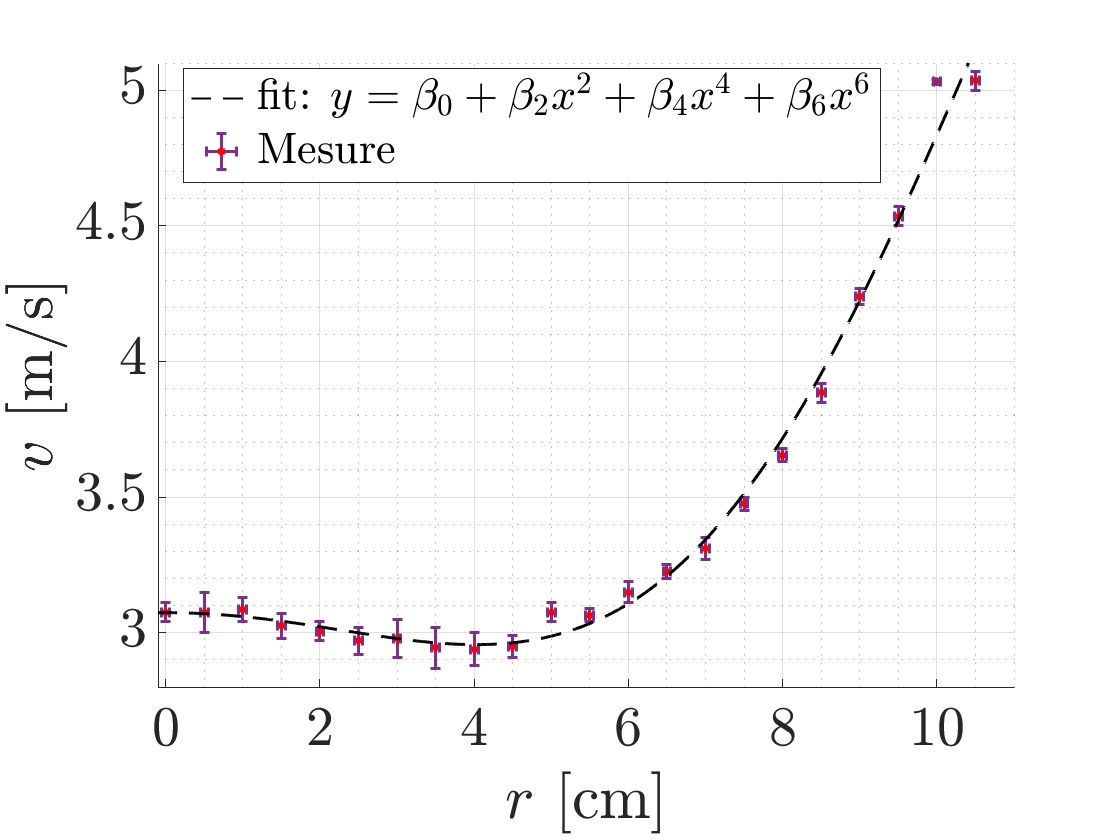
\includegraphics[width=1\linewidth]{fig1re.jpg}
    \captionsetup{justification=centering}
    \caption{Vitesse du fluide pour différentes distances du centre du tube, et fit polynomial de degré 6 donné par $\beta_6 = - (1.8\pm1.0) \times 10^{-6}$ \\
    $\beta_4 = (5.1\pm1.6) \times 10^{-4}$\\
    $\beta_2 = - (0.015\pm0.006)$ \\
    $\beta_0 = (3.07\pm0.06)$}
    \label{fig1re}
\end{wrapfigure}

La Fig.(\ref{fig1re}) illustre le profil de vitesse $v(r)$ mesuré à la sortie du tuyau d’éjection. Les données obtenues ont été ajustées à l’aide d’un polynôme de degré six, avec uniquement des degrés pairs dont les coefficients sont représentés dans le titre de la Fig.(\ref{fig1re}). En intégrant ce profil sur toute la section du tuyau et en utilisant l’équation de continuité hydrodynamique Eq.(\ref{eq5}), la vitesse moyenne $\overline{v}$ dans le tunnel a été déterminée comme suit :  

\vspace{-0.5cm}

\[
\hspace{-0.15cm} \overline{v} = \frac{1}{S_1} \int_0^{2\pi} \hspace{-0.15cm}\int_0^R \hspace{-0.1cm} \left( \beta_6 r^6 + \beta_4 r^4 + \beta_2 r^2 + \beta_0 \right) rdrd\theta
\]

\vspace{-0.2cm}

\[
\overline{v} = \frac{2\pi}{S_1} \int_0^R \left( \beta_6 r^7 + \beta_4 r^5 + \beta_2 r^3 + \beta_0 r \right) dr
\]

\vspace{-0.2cm}

\[
\Rightarrow \overline{v} = \frac{2\pi}{S_1} \left( \frac{\beta_6}{8} R^8 + \frac{\beta_4}{6} R^6 + \frac{\beta_2}{4} R^4 + \frac{\beta_0}{2} R^2 \right) = (5.71\pm0.13)\,\text{m}\cdot\text{s}^{-1}
\]

Enfin, le coefficient de correction $C_\alpha$, reliant cette vitesse moyenne à la vitesse mesurée au centre $v_c$, a été calculé. Avec $v_c = ( 3.07 \pm 0.04) \, \text{m·s}^{-1}$, ce facteur est donné par :

\vspace{-0.25cm}
\[
C_\alpha = \frac{\overline{v}}{v_c} = 1.86 \pm 0.06
\] 
\vspace{-0.35cm}

Ce coefficient a été utilisé dans l’ensemble des expériences pour estimer la vitesse moyenne à partir des mesures de la vitesse centrale.

\vspace{-0.6cm}
\paragraph{Coefficient de pénétration de formes géométriques} 

La Fig.(\ref{fig2}) présente la force de résistance $|\vec{R}|$ en fonction de la vitesse au centre de la sortie au carré $v^2$ de chaque objet. Un fit linéaire a été effectué pour chaque objet, afin de calculer de coefficient $C_x$. Le Tab.(\ref{Tab1}) présente les coefficients des extrapolations affines avec $y(x)=b+a \cdot x$ ainsi que les valeurs calculées de $C_x$ , avec leurs incertitudes, les valeurs de référence et l'erreur relative correspondantes.
\vspace{-0.35cm}

\begin{figure}[H]
    \centering
    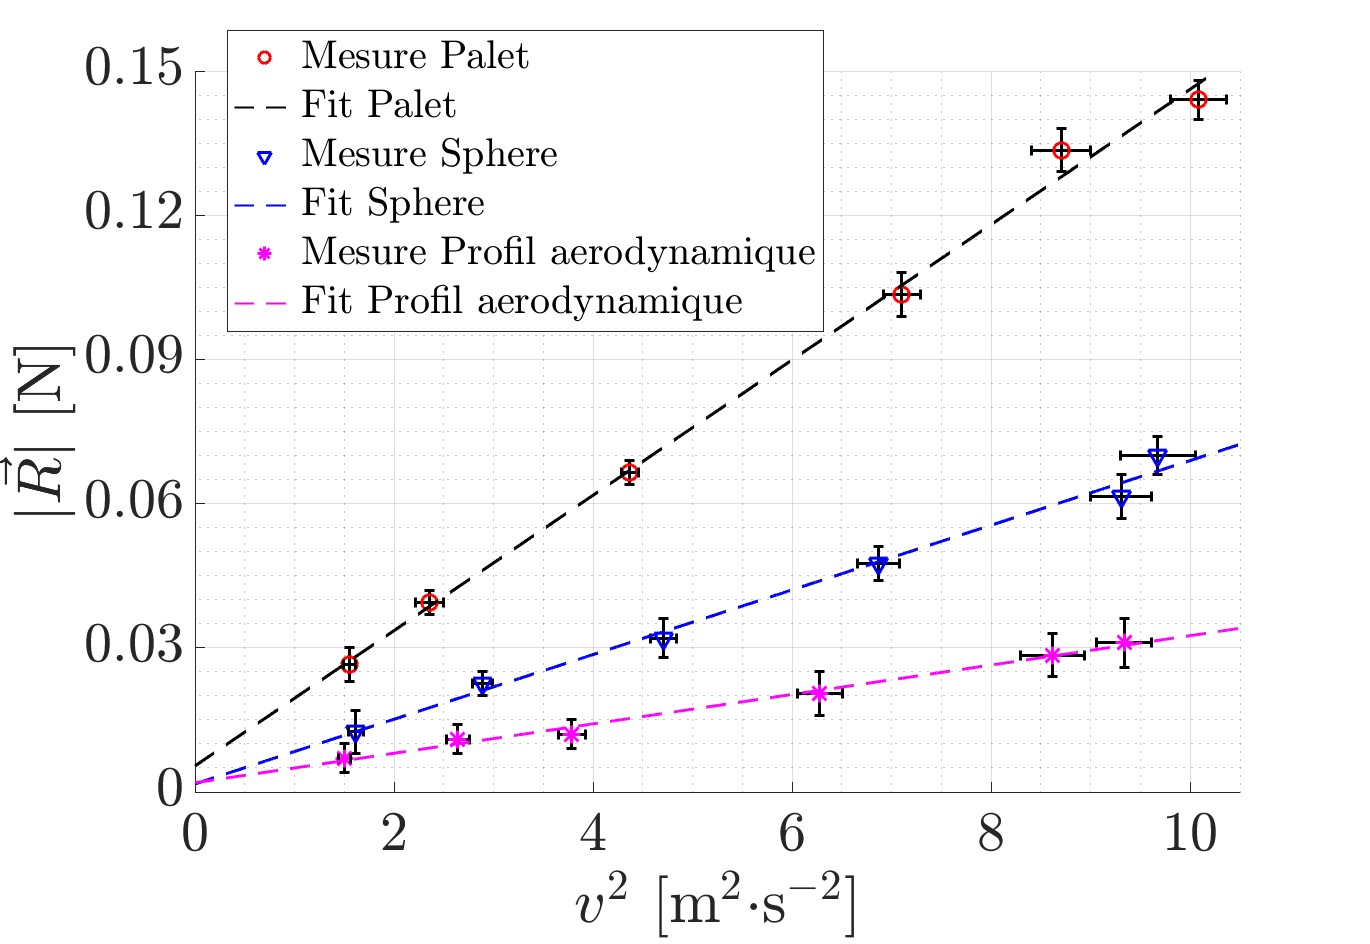
\includegraphics[width=0.6\textwidth]{Graphes/fig2.jpg}
    \captionsetup{justification=centering}
    \caption{Force de résistance $|\vec{R}|$ mesurée sur trois objets à symétrie cylindrique dans une soufflerie en fonction de la vitesse au centre du tuyau d'éjection au carré $v^2$, avec fit linéaire sur les mesures dont les coefficients sont présentés dans le Tab.(\ref{Tab1}).}
    \label{fig2}
\end{figure}

\clearpage

\begin{table}[H]
    \centering
    \renewcommand{\arraystretch}{1.5} % Ajuster la hauteur des lignes
    \setlength{\tabcolsep}{8pt} % Ajuster l'espacement entre les colonnes
    \begin{tabular}{|l|c|c|c|c|c|}
        \hline
        \textbf{} & \textbf{b} & \textbf{a} & \boldmath$C_x$ & \boldmath$C_{x,\text{ref}}$ [\ref{ref3}] & $\varepsilon$ \,[\%]\\ 
        \hline
        Palet &  $(5\pm5) \cdot 10^{-3}$ & $(1.4\pm0.1)\cdot 10^{-2}$ & $2.7\pm0.8$ & 1.1& 150 \\ 
        \hline
        Sphère & $(1\pm5) \cdot 10^{-3}$ & $(6.7\pm0.9)\cdot 10^{-3}$  & $1.3\pm0.7$  & 0.47 & 180 \\ 
        \hline
        Profil aérodynamique & $(2\pm2) \cdot 10^{-3}$ & $(3.1\pm0.3)\cdot 10^{-3}$ & $0.6\pm0.2$ & 0.04 & 1400 \\ 
        \hline
    \end{tabular}
    \captionsetup{justification=centering}
    \caption{Comparaison des coefficients des fits linéaires $a$ et $b$ et des coefficients $C_x$ par rapport à leur valeur de référence $C_{x,\text{ref}}$ [\ref{ref3}] ainsi que l'erreur relative résultante $\varepsilon$.}
    \label{Tab1}
\end{table}

\vspace{0.5cm}

\paragraph{Coefficients de portance et de traînée d’une aile d’avion}  

\begin{wrapfigure}{H}{0.55\textwidth}
    \centering
    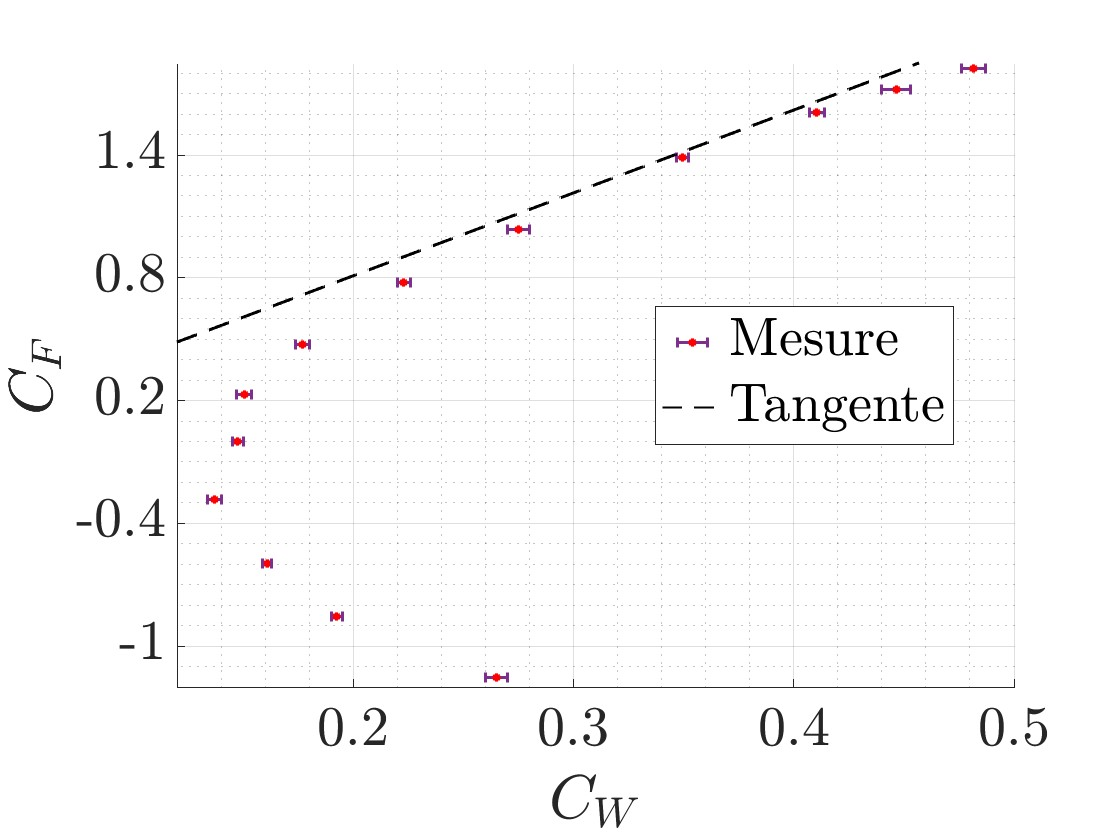
\includegraphics[width=1\linewidth]{Graphes/fig3.jpg}
    \captionsetup{justification=centering}
    \caption{Diagramme de Lilienthal pour $v=(2.90\pm0.05)$m$\cdot$s$^{-1}$.La tangente est décrite par \( y = (4.1 \pm 0.2)x \).}
    \label{fig3}
\end{wrapfigure}

Les coefficients de traînée et de portance ont été calculés à l'aide des équations (\ref{eq4}). La Fig.(\ref{fig3}) présente le diagramme polaire de Lilienthal, montrant les variations des coefficients en fonction de l’angle d’attaque. L’angle optimal maximisant le rapport $C_F/C_W$ a été déterminé à partir de la tangente passant par l’origine, et les résultats indiquent une efficacité aérodynamique maximale pour $\gamma = (12.50 \pm 0.05)$\,°.

\vspace{0.5cm}

\paragraph{Coefficient de pénétration d’une maquette de voiture}  
La force de résistance $|\vec{R}|$ a été mesurée en fonction de $v^2$, et les résultats sont tracés sur la Fig.(\ref{fig4a}), avec un fit linéaire de la forme $y= \alpha x + \beta $, avec $\alpha =(1\pm2)\times 10^{-3}$ et $\beta =(4.4\pm0.4)\times 10^{-3}$ . À partir de la pente $\alpha$, le coefficient $C_x$ a été calculé en utilisant la même méthode que pour les formes géométriques donc la relation (\ref{eq6}) pour une section $S=(32.0\pm0.6)$\,cm$^2$. Le résultat obtenu est $C_x = 0.7\pm0.3$. 

De plus, la force de portance a été mesurée et tracée sur la Fig.(\ref{fig4b}). Ainsi, cela permet de calculer le nombre de Reynolds pour le modèle ainsi que pour la vraie formule 1. Le nombre de Reynolds pour la voiture réelle et le modèle peut être calculé en utilisant l'équation (\ref{eq1}), les longueurs du modèle \( l_{\text{modele}}=(23.00\pm0.05) \times10^{-2}\,\text{m}\) et de la voiture \( l_{\text{voiture}} = (5.50 \pm 0.13) \, \text{m} \)  [\ref{ref6}], ainsi que les vitesses maximales, à savoir \( v_{\text{modele}} = (5.7 \pm 1.0) \, \text{m} \cdot \text{s}^{-1} \) et \( v_{\text{voiture}} = 300 \, \text{km} \cdot \text{h}^{-1} = 83.3 \, \text{m} \cdot \text{s}^{-1} \) [\ref{ref3}]. Cela donne :

\vspace{0.5cm}

\[
\text{Re}_{\text{modele}} = (9.2 \pm 1.6) \times 10^4, \quad \text{Re}_{\text{voiture}} = (3.23 \pm 0.08) \times 10^7
\] 

\begin{figure}[H]
\begin{subfigure}{0.45\textwidth}  % Réduire la taille pour s'assurer qu'elles tiennent côte à côte
    \centering  % Centrer cette sous-figure
    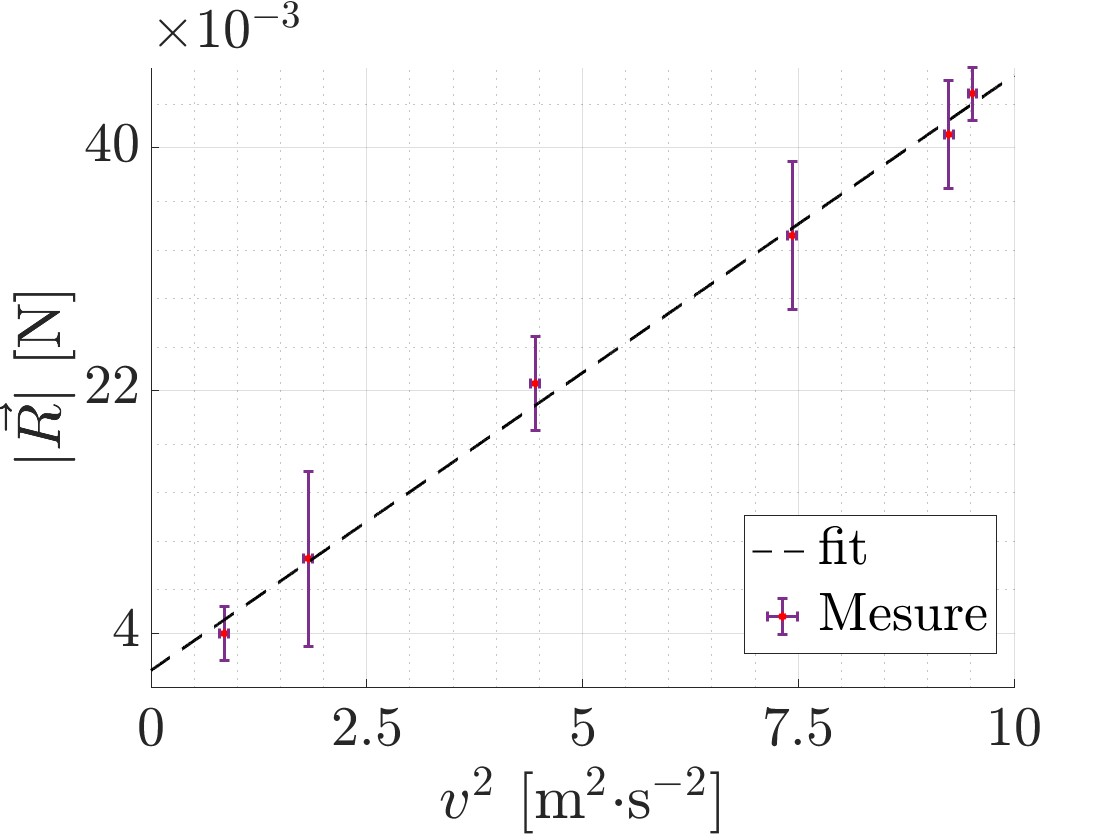
\includegraphics[scale=0.21]{Graphes/fig4.jpg}
    \captionsetup{justification = centering, font=large}
    \caption{}
    \label{fig4a}
\end{subfigure}
\hspace{0.05\textwidth}
\begin{subfigure}{0.45\textwidth}  % Réduire également ici
    \centering  % Centrer cette sous-figure
    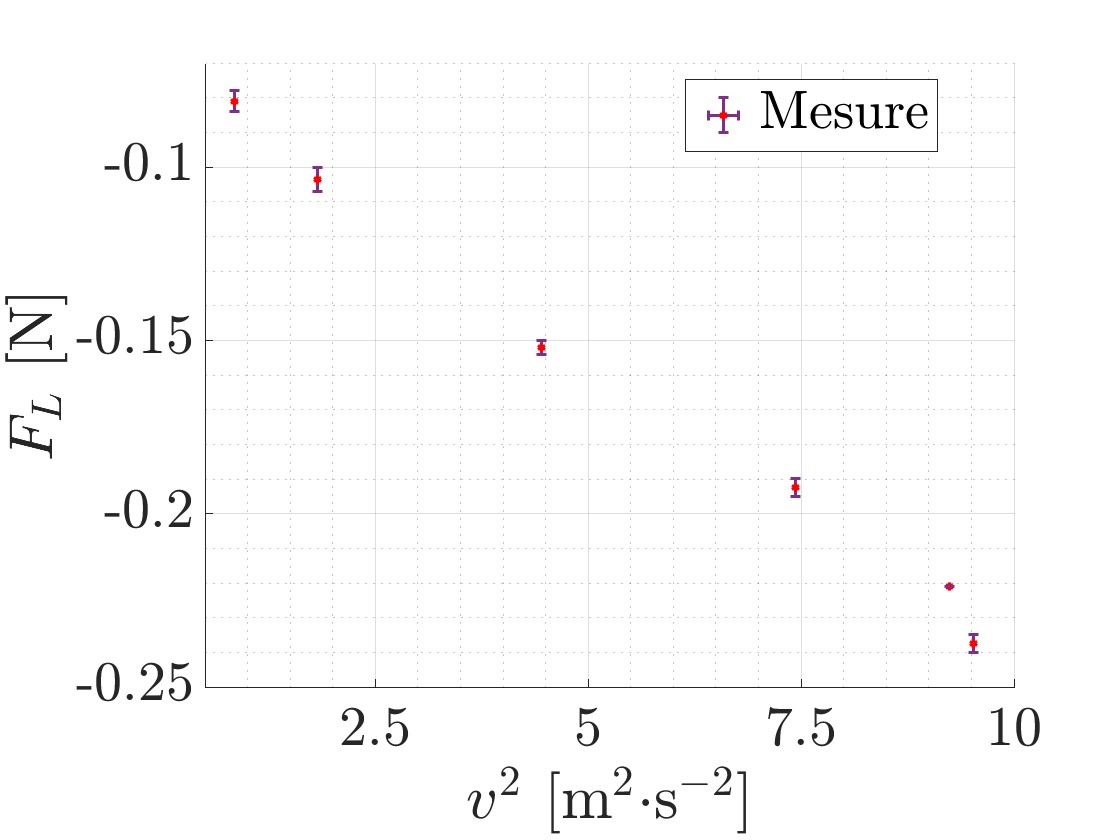
\includegraphics[scale=0.21]{Graphes/fig5.jpg}
    \captionsetup{justification = centering, font=large}
    \caption{}
    \label{fig4b}
\end{subfigure}
\vspace{-0.3cm}
\captionsetup{justification=centering}
\caption{(a) Force de résistance $|\vec{R}|$ et (b) Force de portance $F_L$ mesurées sur un modèle de formule 1 placée dans une soufflerie en fonction de la vitesse au centre de la sortie au carré $v^2$.}
\label{fig1}
\end{figure}

\section{Discussion}

\paragraph{Détermination du profil de vitesse dans le tunnel aérodynamique}

La calibration du profil de vitesse a permis d’obtenir une estimation de la vitesse moyenne d’écoulement dans le tunnel aérodynamique, basée sur l’hypothèse d’une symétrie cylindrique du flux. Néanmoins, cette hypothèse pourrait être invalidée par des écarts locaux dans la vitesse dus à des turbulences résiduelles ou des défauts de fabrication du conduit déformant le cylindre. C'est pourquoi une grosse erreur a été choisie pour le choix du rayon de la bouche de sortie. Outre la forme pas parfaitement cylindrique, remettant en cause le calcul par intégrale de la vitesse moyenne, ces déformations génèrent des variations de flux de vitesse non négligeables. De plus, l’utilisation d’un anémomètre placé au centre du flux introduit une incertitude. Les variations locales de la vitesse, en dehors du centre du cylindre, ne sont pas parfaitement capturées. Une amélioration notable pourrait être d’effectuer des mesures à l’aide d’un anémomètre laser Doppler [\ref{ref7}], permettant une caractérisation plus fine et sans contact du champ de vitesse. Par ailleurs, un élargissement de la grille de points de mesure sur toute la section de sortie permettrait de vérifier davantage l’hypothèse de symétrie et de détecter les asymétries. Bien que les limitations mentionnées puissent introduire des biais, le facteur \(C_\alpha\) reste une approximation fiable dans le cadre des expériences ultérieures.

\paragraph{Étude du coefficient de pénétration des formes géométriques}

L’évaluation des coefficients de pénétration $C_x$ pour différentes formes géométriques a confirmé que la force de traînée est proportionnelle au carré de la vitesse moyenne, comme attendu. Les objets optimisés aérodynamiquement, tel que le profil aérodynamique, affichent un $C_x$ sensiblement plus faible que les formes plus rudimentaires, comme le palet par exemple. Cette distinction reflète bien l’impact de la géométrie sur la formation des turbulences à l’arrière des obstacles. Cependant, les résultats diffèrent grandement des attentes théoriques, en effet, les erreurs relatives sur les coefficients $C_x$ sont de 150\%, 180\% et 1400\% pour le palet, la sphère et le profil aérodynamique respectivement. Ceci peut être expliqué par plusieurs facteurs influençant la précision des mesures. Tout d’abord, les forces parasites générées par les supports des objets introduisent une contribution non négligeable aux mesures de traînée. Les tiges de support, bien qu’étroites, perturbent le flux et ajoutent une traînée qui modifie et amplifie le calcul de $C_x$. Ensuite, les capteurs de force, bien qu’efficaces, présentent une certaine imprécision, amplifiée par des fluctuations du flux. Une estimation plus exacte des coefficients de pénétration pourrait être effectuée en répétant les mesures pour plus de vitesses différentes et en utilisant un équipement de mesure plus précis. Ces écarts pourraient être aussi attribués à des approximations dans le calcul du $C_\alpha$, ou à des hypothèses simplifiées sur la section efficace des objets.

\paragraph{Caractérisation des coefficients de traînée et de portance d’une aile}

L’analyse de l’aile d’avion a permis de tracer un diagramme de Lilienthal, montrant que le rapport $C_F/C_W$ est maximal pour un angle d’attaque optimal d’environ $(12.50\pm0.05)$\,°. Ce résultat illustre clairement l’importance de la géométrie de l’aile et de l’ajustement de son inclinaison pour maximiser les performances aérodynamiques. Cependant, plusieurs limitations techniques et expérimentales peuvent affecter les conclusions. En premier lieu, les capteurs de force utilisés pour mesurer la portance et la traînée présentent toujours une imprécision. Les fluctuations des forces en régime turbulent pourraient être mieux capturées à l’aide d’un système de mesure plus sensible, comme un capteur à fibre optique [\ref{ref8}]. Enfin, la simplification du modèle de l’aile peut entraîner des limitations. Une étude complémentaire pourrait inclure des variations de la géométrie de l’aile : épaisseur, rapport longueur/profondeur. Ceci permettrait d'évaluer l'influence de la géométrie de l'aile sur les coefficients aérodynamiques. Enfin, l’utilisation d’un flux plus uniforme dans le tunnel, par exemple grâce à des grilles de stabilisation en amont, permettrait de minimiser les fluctuations non désirées.

\paragraph{Étude du coefficient de pénétration d’une maquette de Formule 1}

L’étude aérodynamique de la maquette de Formule 1 a révélé que le coefficient de pénétration $C_x$ peut être mesuré pour des vitesses modérées. Néanmoins, les résultats montrent que le nombre de Reynolds de l’écoulement autour de la maquette est inférieur de plusieurs ordres de grandeur à celui de la voiture réelle. Cela rend difficile toute extrapolation directe des résultats à l’échelle réelle. Pour remédier à ce problème, une première idée serait d'augmenter la vitesse d'écoulement du fluide dans la soufflerie. Cependant, pour trouver des nombres de Reynolds similaires entre la maquette et la formule 1 réelle, il faudrait une vitesse d'écoulement supérieure à la vitesse du son. Cela paraît naturellement inenvisageable, et d'autres solutions doivent être explorées. Par exemple, remplacer l’air par un fluide plus dense, comme l’eau, permettrait d’augmenter le nombre de Reynolds tout en maintenant des vitesses de flux raisonnables. Une autre approche serait d’augmenter l’échelle de la maquette, bien que cela implique des contraintes techniques importantes dans la soufflerie. Par ailleurs, la mesure de la force de portance négative, due à la géométrie de la voiture, souligne l’importance des appendices aérodynamiques pour maintenir l’adhérence au sol, et est un rôle clé dans le développement de telles voitures. Une amélioration de l’expérience pourrait inclure l’étude de différentes configurations des ailerons de la voiture afin d'évaluer leur impact sur la stabilité dynamique du véhicule.

\section{Conclusion}

Ce travail a permis d’explorer plusieurs aspects fondamentaux de l’aérodynamique en combinant analyse théorique et observations expérimentales. La calibration du flux de vitesse dans le tunnel a fourni une base solide pour interpréter les données, malgré certaines simplifications. L’étude des formes géométriques a confirmé l’influence majeure de la géométrie sur la traînée, démontrant que les objets profilés présentent des performances bien supérieures en termes de pénétration. L’analyse des coefficients de portance et de traînée d’une aile a mis en évidence l’importance de l’angle d’attaque, soulignant l’équilibre subtil nécessaire pour maximiser l’efficacité aérodynamique. Enfin, l’évaluation d’une maquette de Formule 1 a illustré les défis liés aux études à échelle réduite, tout en mettant en lumière le rôle essentiel des dispositifs comme les ailerons dans la stabilité dynamique. Ce TP a permis d'approfondir la compréhension de l'aérodynamique ainsi que des limites des approches expérimentales à ce sujet. Une réflexion pourrait également être engagée sur les implications environnementales des performances aérodynamiques, un sujet essentiel dans le contexte actuel de transition énergétique, où réduire la traînée signifie aussi limiter la consommation d’énergie [\ref{ref9}].

\section*{Annexe}

\subsection*{Références}
\renewcommand{\labelenumi}{[\theenumi]}
\begin{enumerate}

    \item \label{ref1} DefTechClub, Comment l’aérodynamique avancée révolutionne-t-elle le transport du futur ?\\
    \url{https://deftechclub.com/comment-laerodynamique-avancee-revolutionne-t-elle-le-transport-du-futur/}
    \item \label{ref2} AmusementLogic, L’aérodynamique dans l’architecture et la construction\\
    \url{https://amusementlogic.fr/nouvelles-generales/laerodynamique-dans-larchitecture-et-la-construction/}
    \item \label{ref3} EPFL, TP de Physique B1, Aérodynamique
    \url{https://epflch.sharepoint.com/sites/sph-ge/Documents%20partages/Forms/AllItems.aspx?id=%2Fsites%2Fsph-ge%2FDocuments%20partages%2FWebsiteSPH%2FNotices%2FTP2%2FFR%2FB1_Aérodynamique%2Epdf&parent=%2Fsites%2Fsph-ge%2FDocuments%20partages%2FWebsiteSPH%2FNotices%2FTP2%2FFR&p=true&ga=1}
    \item \label{ref4} Wikipedia, Masse volumique de l'air, consulté le 09/12/2024
    \url{https://fr.wikipedia.org/wiki/Masse_volumique_de_l%27air}
    \item \label{ref5}Flottweg, Viscosité dynamique (coefficient de frottement interne)\\
    \url{https://www.flottweg.com/fr/wiki/separation-technology/viscosite-dynamique/}
    \item \label{ref6} Motorsport, Et si les formules 1 retrouvaient leur taille de guêpe?\\
    \url{https://fr.motorsport.com/f1/news/si-f1-retrouvaient-taille-guepe/10454765/#:~:text=La%20longueur%20passe%20donc%20de,reste%20comparable%20aux%20enveloppes%20modernes.}
    \item \label{ref7} OPI, Anémométrie Laser Doppler (ALD) et Vélocimétrie Laser Doppler (VLD)\\
    \url{http://www.optique-ingenieur.org/fr/cours/OPI_fr_M02_C08/co/Contenu_06.html}
    \item \label{ref8} Eduscol, Capteurs à fibres optiques : principe de fonctionnement\\
    \url{https://eduscol.education.fr/sti/sites/eduscol.education.fr.sti/files/ressources/pedagogiques/15992/15992-capteurs-fibres-optiques-principe-de-fonctionnement-ensps.pdf}
    \item \label{ref9} Toyota, Quel impact l’aérodynamisme a-t-il sur la consommation de carburant?\\
    \url{https://www.toyota.ca/toyota/fr/connect/1003/quel-impact-laerodynamisme-a-t-il-sur-la-consommation-de-carburant}


\end{enumerate}

$\gamma=(12.50\pm0.05)$\,°

\subsection*{Incertitudes}
\paragraph{Vitesse moyenne du flux}

L'erreur sur la vitesse moyenne du flux $\overline{v}$, donnée par l'équation (\ref{ref5}), est calculée comme suit :
\begin{equation}
    \Delta \overline{v} = \frac{\overline{v}}{S_1} \Delta S_1 + \left| \frac{2\pi}{S_1} \left(\beta_6 R^8 + \beta_4 R^6 +\beta_2 R^4 +\beta_0 R^2 +\right) \Delta R \right|
\end{equation}

\noindent avec l'erreur sur la section transversale de la soufflerie $S_1 = h l$ donnée par :
\begin{equation}
    \Delta S_1 = |l \Delta h| + |h \Delta l|
\end{equation}

L'erreur sur le facteur de correction $C_\alpha = \frac{\overline{v}}{v_c}$ est donnée par :
\begin{equation}
    \Delta C_\alpha = \left| \frac{\Delta \overline{v}}{v_c} \right| + \left| \frac{C_\alpha}{v_c} \Delta v_c \right|
\end{equation}

Enfin, l'erreur sur la vitesse moyenne $\overline{v}$, définie par $\overline{v} = C_\alpha v_c$, est calculée comme suit :
\begin{equation}
    \Delta \overline{v} = \left| v_c \Delta C_\alpha \right| + \left| C_\alpha \Delta v_c \right|
\end{equation}

\paragraph{Coefficient de pénétration}

L'erreur sur le coefficient de pénétration $C_x = \frac{2a}{\rho S}$ avec $a$ le coefficient du fit linéaire de la Fig.(\ref{fig2}) et la Fig.(\ref{fig4a}) est donnée par :
\begin{equation}
    \Delta C_x = \left| \frac{2}{\rho S} \Delta a \right| + \left| \frac{C_x}{S} \Delta S \right|
\end{equation}

avec l'erreur sur l'aire apparente $S = \pi r^2$ donnée par :
\begin{equation}
    \Delta S = \left| 2\pi r \Delta r \right|
\end{equation}

L'erreur sur la pente $a$ est obtenue sur MATLAB avec un intervalle de confiance de 95\%.

\paragraph{Nombre de Reynolds}

L'erreur sur le nombre de Reynolds $Re$, donné par l'équation (\ref{eq1}), est calculée comme suit :
\begin{equation}
    \Delta Re = \left| \frac{Re}{v} \Delta v \right| + \left| \frac{Re}{l} \Delta l \right|
\end{equation}


\end{document}